\subsection{Lilian Kennedy}
Having recently transferred courses, Lilian had to learn a lot in a short period of time. She had to learn the fundamentals of website development while implementing the front-end. She became familiar with the basics of HTML and CSS through her first trial of building the website as shown in figure \ref{fig:initial}. \\

However she felt there was more potential for the front-end of the project. This resulted in a complete redesign of the website as shown in figure \ref{fig:plan}. This delayed development but improved the quality of the user interface. Utilising what she had learnt from her initial website, she was able to develop a new and improved website. Lilian struggled with the learning curve of JavaScript, which was vital for the interconnectivity of the project. She was able to reach out to her teammates for help and support.\\


\begin{figure}[!ht]
    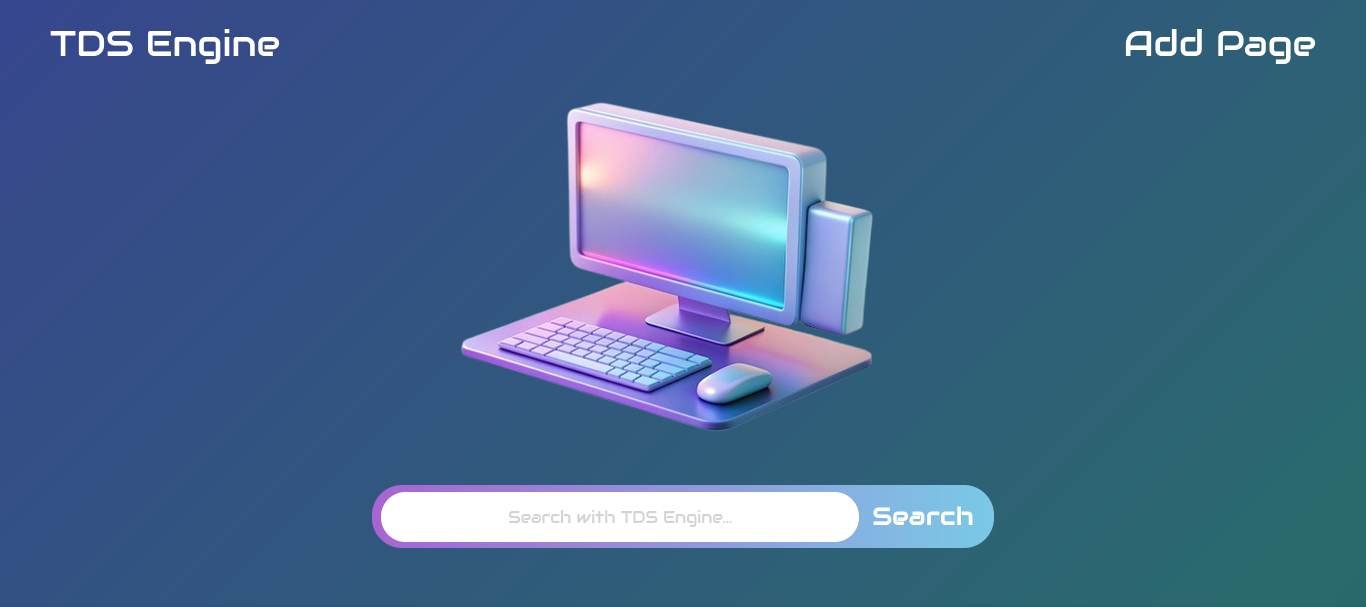
\includegraphics[width=\textwidth,keepaspectratio]{old-website.png}\\
    \caption{Initial Website}
    \label{fig:initial}
\end{figure}

\newpage

\begin{figure}[!ht]
    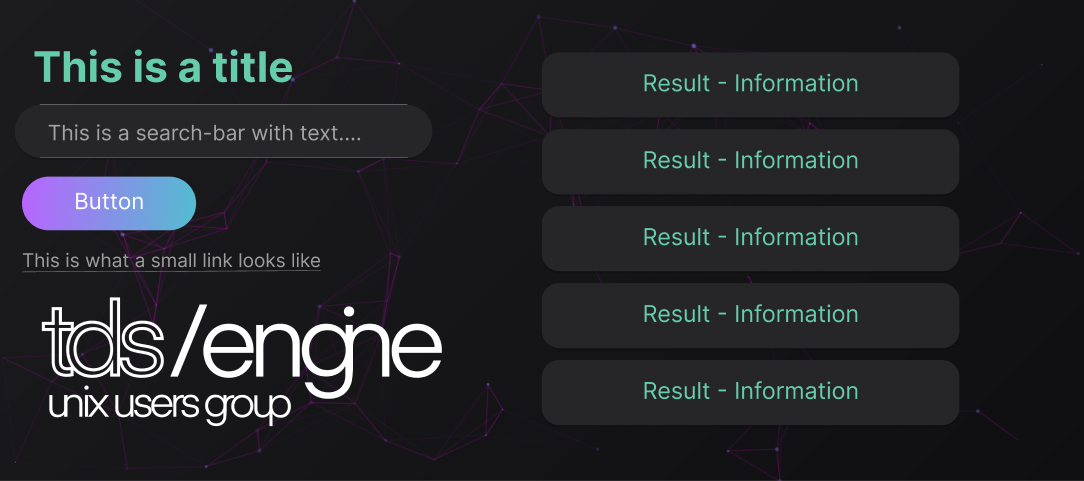
\includegraphics[width=\textwidth,keepaspectratio]{design-plan.png}\\
    \caption{Website Design Plan, demonstrating importance of coherence in UI design}
    \label{fig:plan}
\end{figure}
